\section{Experimental Evaluation}
\label{sec:eval}
The evaluation considers fallback-free placement, deployed accuracy,
engine-plus-transfer latency, application-pipeline latency, and module energy
at a matched delivered
rate; engine hashes, per-image predictions, timing records, and power traces
connect the compiled configurations to measured behavior. Each precision mode
includes stock YOLO11n on GPU and with DLA+GPU fallback (stock fallback), and \model\ on GPU
and strict DLA. Tables abbreviate these models as 11n and 11-DLA; DLA denotes
strict placement for the adapted model.

\subsection{Platform and Precision Protocol}
\label{sec:setup}
Tests use an NVIDIA Jetson AGX Orin Developer Kit with L4T 36.4.4, CUDA runtime
12.6, TensorRT 10.3.0, PyTorch 2.5.0a0, and ROS~2 Jazzy. The platform is
configured in NVIDIA's 50\,W power mode with \texttt{jetson\_clocks} disabled;
CPU frequencies vary during measurement. Strict execution targets DLA core 0,
and the benchmark is a standalone runner rather than a ROS~2 node.
All configurations use batch one and $640\times640$ inputs. FP16 enables
half precision; INT8 enables both INT8 and FP16. These names describe build
modes, not uniform precision of every operation: GPU regions may retain
FP16/FP32 intermediates.

Post-training calibration uses 500 COCO val2017 images sampled without
replacement with seed 2027, leaving 4,500 disjoint images for accuracy
\cite{lin2014coco}. The two ONNX models have separate entropy-calibration
caches, generated before fusion with TensorRT's EntropyCalibrator2 using the
same image IDs, batch one, and normalized FP32 RGB letterboxed inputs.
No labels enter calibration, and INT8 entails no additional training. Each
model's cache is shared across its GPU and DLA placements. The calibrated
engines and native I/O scales are validated before evaluation.

\subsection{Fallback-Free Placement}
\label{sec:placement}
Stock YOLO11n fails strict FP16 compilation at its attention MatMul; no
fallback-disabled stock INT8 build was attempted. The
adapted FP16 build assigns 299 layers to DLA and none to GPU. Both adapted
strict engines have one optimized DLA node corresponding to one loadable,
with no GPU or reformat nodes. The INT8 build assigns 298 layers to INT8 and
one softmax to FP16, all on DLA. Fallback-disabled compilation and inspection
therefore satisfy Eq.~\eqref{eq:accept} for both tested precision modes;
fallback-free does not imply integer-only computation.

The stock FP16 fallback engine instead contains four DLA loadables, eleven GPU
compute nodes, twenty-two reformats, and ten no-op/constant nodes. Its separate
layer profile attributes 93.97\% of time to DLA, 4.73\% to reformats, and
1.30\% to GPU computation (Fig.~\ref{fig:profile}); the summed device profile
is 34.312\,ms, including 32.244\,ms in DLA segments. Stock INT8 fallback also
has four DLA loadables, with twenty-three reformats among 48 optimized nodes.
Comparing these heterogeneous deployments with strict DLA includes changed
attention and output boundaries and does not isolate partitioning cost.

\begin{figure}[t]
\centering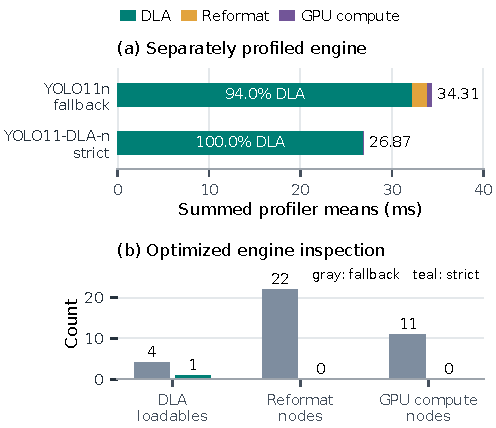
\includegraphics[width=\columnwidth]{figures/fallback_profile.pdf}
\caption{FP16 placement and separate layer profiles. Stock fallback has four
DLA loadables and intervening GPU/reformat work; the adapted strict engine has
one DLA loadable. These time shares characterize FP16, not INT8.}
\label{fig:profile}
\end{figure}

\subsection{Engine-Plus-Transfer Latency and Throughput}
\label{sec:engine}
The \texttt{trtexec} microbenchmark uses a 2\,s warm-up, a 30\,s timing window,
one inference stream, spin waiting, generated input data, and transfers enabled:
\begin{equation}
 L_{\mathrm{engine+IO}}=T_{\mathrm{H2D}}+T_{\mathrm{device}}+T_{\mathrm{D2H}}.
 \label{eq:latency}
\end{equation}
This boundary excludes preprocessing, host-side decoding, and NMS. TensorRT's
``GPU Compute Time'' field measures device execution even for a DLA engine;
it does not establish GPU computation. Query throughput uses host wall time
and can differ from reciprocal median latency because transfers and execution
overlap. Profiles are collected separately. P95 and P99 characterize frame
variation within tests, not confidence intervals across independent trials.

\begin{table}[t]
\caption{Engine-plus-transfer latency, batch one, $640\times640$. Median and P95 are milliseconds; rate is queries/s.}
\label{tab:engine}\centering\footnotesize
\setlength{\tabcolsep}{3pt}
\begin{tabular*}{\columnwidth}{@{\extracolsep{\fill}}llrrr@{}}
\toprule
Model / device & Mode & Median & P95 & Rate \\
\midrule
11n / GPU & FP16 & 3.740 & 3.753 & 288.3 \\
11n / DLA+GPU & FP16 & 34.678 & 34.942 & 29.2 \\
11-DLA / GPU & FP16 & 3.500 & 3.512 & 317.2 \\
11-DLA / DLA & FP16 & 27.515 & 27.718 & 37.2 \\
\midrule
11n / GPU & INT8 & 3.021 & 3.030 & 357.0 \\
11n / DLA+GPU & INT8 & 13.068 & 13.094 & 79.5 \\
11-DLA / GPU & INT8 & 2.828 & 2.836 & 393.4 \\
11-DLA / DLA & INT8 & 4.167 & 4.173 & 263.7 \\
\bottomrule
\end{tabular*}
\end{table}

\begin{figure}[t]
\centering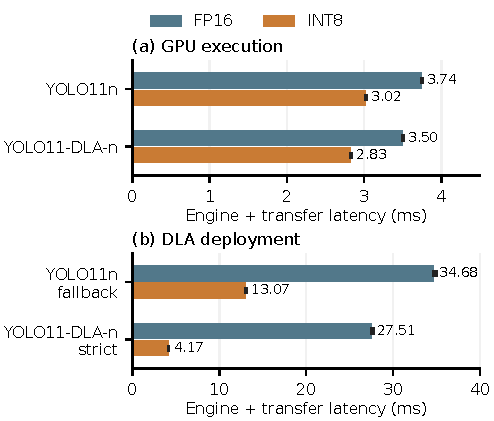
\includegraphics[width=\columnwidth]{figures/precision_latency.pdf}
\caption{FP16 and INT8 engine-plus-transfer latency. Bars show medians and
whiskers extend to P95; panels use different horizontal scales. INT8 provides
a larger relative reduction for strict DLA than for the GPU controls.}
\label{fig:latency}
\end{figure}

Table~\ref{tab:engine} and Fig.~\ref{fig:latency} show that INT8 reduces strict DLA
median engine-plus-transfer latency from 27.515 to 4.167\,ms, a $6.60\times$ speedup, and increases
throughput from 37.2 to 263.7 queries/s. Strict DLA has lower
engine-plus-transfer latency than stock fallback in both modes: 20.7\% lower
median in FP16 and a $3.14\times$ reduction in INT8. The same adapted model on
GPU remains faster at this boundary: 3.500\,ms in FP16 and 2.828\,ms in INT8. Strict INT8 device execution alone
is 3.789\,ms. Neither result establishes comparable accuracy or application
performance.

\subsection{Deployed-Engine Accuracy}
\label{sec:accuracy}
The main comparison evaluates all eight configurations on the same 4,500
held-out IDs, verifying matching image hashes. FP16 predictions from the
existing 5,000-image evaluation are rescored on this subset without rerunning
inference. Preprocessing centers a square $640\times640$ letterbox with padding
114 and RGB normalization by 255. CPU post-processing uses confidence 0.001,
class-aware NMS at intersection over union (IoU) 0.7, multi-label candidates,
and at most 300 boxes per image; COCOeval uses standard detection limits.
These settings differ from the timing thresholds.

\begin{table}[t]
\caption{Accuracy on 4,500 held-out COCO val2017 images, disjoint from INT8 calibration. AP values are percentage points; INT8 allows mixed precision; stock and adapted training budgets differ.}
\label{tab:accuracy}\centering\footnotesize
\setlength{\tabcolsep}{3pt}
\begin{tabular*}{\columnwidth}{@{\extracolsep{\fill}}llrrr@{}}
\toprule
Model / device & Mode & AP & AP$_{50}$ & AP$_{75}$ \\
\midrule
11n / GPU & FP16 & 39.378 & 55.190 & 42.845 \\
11n / DLA+GPU & FP16 & 39.308 & 55.160 & 42.823 \\
11-DLA / GPU & FP16 & 37.879 & 53.633 & 41.008 \\
11-DLA / DLA & FP16 & 37.876 & 53.614 & 41.016 \\
\midrule
11n / GPU & INT8 & 33.175 & 47.324 & 36.069 \\
11n / DLA+GPU & INT8 & 19.827 & 35.241 & 20.867 \\
11-DLA / GPU & INT8 & 35.951 & 51.063 & 39.323 \\
11-DLA / DLA & INT8 & 35.408 & 50.790 & 38.614 \\
\bottomrule
\end{tabular*}
\end{table}

Table~\ref{tab:accuracy} separates precision loss from placement effects.
Strict INT8 loses 2.468 AP points relative to strict FP16; adapted GPU loses
1.928 points. Within a precision mode, strict DLA minus adapted GPU AP is
$-0.003$ points in FP16 and $-0.543$ in INT8. Thus, the negligible FP16
placement difference does not extend unchanged to INT8.
Stock GPU loses 6.203 points, while stock fallback loses 19.48 AP points,
reaching only 19.827 AP. Under this calibration protocol the adapted INT8
engines exceed stock INT8 accuracy, but the fallback result is not an
accuracy-equivalent baseline: its degradation has no isolated causal
explanation here, and architecture, training, and calibration differences
preclude a general claim about quantization robustness.

The original full-5,000-image FP16 AP values are 39.314 (stock GPU), 39.245
(stock fallback), 37.995 (adapted GPU), and 37.991 (strict DLA); they must not
be compared directly with held-out INT8 AP.
The adapted checkpoint's stored 500-epoch validation history ends at AP 37.581
and AP$_{50}$ 53.151 under a different evaluation protocol; these training
metrics do not establish an export-induced gain.

\subsection{Export, Layout, and Decoder Checks}
\label{sec:parity}
A CPU check on one random input (seed 7) finds maximum external-decoder error
$1.22\times10^{-4}$ and raw-map ONNX/checkpoint error $3.07\times10^{-4}$;
these are distinct from engine validation. On 50 real images, each
precision campaign passes eight layout checks and 200 dense/sparse decoder
comparisons: two engines and two confidence settings (0.001 multi-label and
0.25 single-label). The exploratory raw GPU/DLA comparison, at absolute
and relative tolerances 0.1 and 0.05, fails on 50/49/49 images for FP16
P3/P4/P5 and on all 50 at every level for INT8. Raw agreement is therefore
reported diagnostically, not claimed as a passed numerical gate.

On all 5,000 images, FP16 dense/sparse AP differs by less than $10^{-7}$
points; one GPU image (74092) has 252 sparse versus 251 dense detections.
On the 4,500 held-out images, INT8 dense/sparse AP is identical at reported
precision for both adapted engines, but GPU image 408774 has 295 sparse
versus 294 dense detections. Aggregate accuracy agreement does not establish
bitwise identity or equality of every post-NMS detection.

\subsection{Multi-Image Application Pipeline}
\label{sec:application}
The sequential runtime preloads the same first 100 validation images in sorted
ID order for both precisions, then cycles through them for 60\,s after 30
warm-up frames and 30\,s stabilization. CPU preprocessing and NMS use one
thread, confidence 0.25, single-label candidates, and NMS IoU 0.45; adapted
engines use sparse decoding.
The boundary includes native I/O and any quantization/dequantization, and
excludes disk access, visualization, camera acquisition, and ROS transport.
Faster configurations complete more cycles within the fixed duration.

\begin{table*}[t]
\caption{Application pipeline on the same 100 images, 60\,s per test. Latency: ms; rate: frames/s. Includes preprocessing, native I/O, inference, decode and NMS.}
\label{tab:e2e}\centering\footnotesize
\setlength{\tabcolsep}{4pt}
\begin{tabular*}{\textwidth}{@{\extracolsep{\fill}}lrrrrrrrr@{}}
\toprule
& \multicolumn{4}{c}{FP16} & \multicolumn{4}{c}{INT8} \\
\cmidrule(lr){2-5}\cmidrule(l){6-9}
Model / device & Median & P95 & P99 & Rate & Median & P95 & P99 & Rate \\
\midrule
11n / GPU & 20.030 & 24.658 & 27.702 & 47.99 & 17.556 & 22.104 & 23.681 & 54.70 \\
11n / DLA+GPU & 51.241 & 59.542 & 64.478 & 18.95 & 29.020 & 37.510 & 40.293 & 32.71 \\
11-DLA / GPU & 20.307 & 24.584 & 28.591 & 47.63 & 18.212 & 22.467 & 23.780 & 53.00 \\
11-DLA / DLA & 56.820 & 65.042 & 76.886 & 17.19 & 30.675 & 34.812 & 36.322 & 31.93 \\
\bottomrule
\end{tabular*}
\end{table*}

INT8 reduces strict DLA median application-pipeline latency from 56.820 to 30.675\,ms,
a $1.85\times$ speedup (Table~\ref{tab:e2e}). This is substantially smaller
than the engine speedup. Strict INT8 input packing/quantization/H2D has median
7.463\,ms, inference 4.522\,ms, output transfer/unpacking/dequantization
10.729\,ms, and post-processing 4.628\,ms. Stock INT8 fallback has corresponding
medians 2.318, 13.467, 1.500, and 5.830\,ms. Native I/O processing thus remains
a substantial cost in this implementation. Stage medians do not sum to median
total latency, and the inference stage includes runtime-call and synchronization
overhead beyond device execution.

The engine ordering reverses at the application boundary in both modes:
strict latency exceeds fallback by 10.9\% in FP16 and 5.7\% in INT8. Adapted
INT8 GPU is faster still, at 18.212\,ms. Host effects also vary: INT8 median
preprocessing is 2.954\,ms for strict DLA versus 5.568\,ms for fallback on
the same images. These tests characterize the observed runtime rather than
isolating hardware costs.

\subsection{Module Energy at a Matched Delivered Rate}
\label{sec:energy}
Energy tests schedule the same 100-image cycle at 10\,Hz for 60\,s, with the
application thresholds and warm-up/stabilization protocol above. Every active
configuration completes 600 frames, six per image, without observed drops or
misses of the 100\,ms release-to-result deadline.

\texttt{tegrastats} samples are requested every 100\,ms and timestamped using
the host monotonic clock upon arrival. Module power sums the non-overlapping \texttt{VDD\_GPU\_SOC},
\texttt{VDD\_CPU\_CV}, and \texttt{VIN\_SYS\_5V0} rails, excluding wall-plug
and whole-carrier consumption. Trapezoidal integration interpolates window
endpoints:
\begin{equation}
 E_{\mathrm{frame}}=\frac{\int_{t_0}^{t_1}P_{\mathrm{module}}(t)\,dt}
 {N_{\mathrm{completed}}}.
 \label{eq:energy}
\end{equation}
Samples bracket every window, with gaps below 0.113\,s; sensor-to-host delay
is not calibrated. Separate idle measurements are 7.002\,W for FP16 and
7.001\,W for INT8, subtracted over each active interval for incremental energy.

\begin{table}[t]
\caption{Module energy at 10\,Hz, 600 frames per test. Power: W; total and idle-subtracted energy: J/frame.}
\label{tab:energy}\centering\footnotesize
\setlength{\tabcolsep}{3pt}
\begin{tabular*}{\columnwidth}{@{\extracolsep{\fill}}llrrr@{}}
\toprule
Model / device & Mode & Power & Total & Incr. \\
\midrule
11n / GPU & FP16 & 7.605 & 0.761 & 0.060 \\
11n / DLA+GPU & FP16 & 9.166 & 0.917 & 0.216 \\
11-DLA / GPU & FP16 & 7.606 & 0.761 & 0.060 \\
11-DLA / DLA & FP16 & 8.738 & 0.874 & 0.174 \\
\midrule
11n / GPU & INT8 & 7.599 & 0.760 & 0.060 \\
11n / DLA+GPU & INT8 & 7.961 & 0.796 & 0.096 \\
11-DLA / GPU & INT8 & 7.599 & 0.760 & 0.060 \\
11-DLA / DLA & INT8 & 8.062 & 0.806 & 0.106 \\
\bottomrule
\end{tabular*}
\end{table}

Strict INT8 uses 0.806\,J/frame, 7.7\% below strict FP16, but 6.1\% above
adapted INT8 GPU (Table~\ref{tab:energy}). Whereas strict FP16 uses 4.7\% less
energy than stock FP16 fallback, strict INT8 is slightly higher than its
fallback counterpart (0.796\,J/frame), whose accuracy is much lower.
GPU module energy remains approximately 0.760--0.761\,J/frame in both modes.
These observations characterize the measured 10\,Hz operating point; small
differences and idle-subtracted values remain sensitive to baseline stability.
